% this is a simplified version of 
% https://github.com/yihui/knitr/blob/master/inst/examples/knitr-beamer.Rnw
\documentclass{beamer}\usepackage[]{graphicx}\usepackage[]{color}
%% maxwidth is the original width if it is less than linewidth
%% otherwise use linewidth (to make sure the graphics do not exceed the margin)
\makeatletter
\def\maxwidth{ %
  \ifdim\Gin@nat@width>\linewidth
    \linewidth
  \else
    \Gin@nat@width
  \fi
}
\makeatother

\definecolor{fgcolor}{rgb}{0.345, 0.345, 0.345}
\newcommand{\hlnum}[1]{\textcolor[rgb]{0.686,0.059,0.569}{#1}}%
\newcommand{\hlstr}[1]{\textcolor[rgb]{0.192,0.494,0.8}{#1}}%
\newcommand{\hlcom}[1]{\textcolor[rgb]{0.678,0.584,0.686}{\textit{#1}}}%
\newcommand{\hlopt}[1]{\textcolor[rgb]{0,0,0}{#1}}%
\newcommand{\hlstd}[1]{\textcolor[rgb]{0.345,0.345,0.345}{#1}}%
\newcommand{\hlkwa}[1]{\textcolor[rgb]{0.161,0.373,0.58}{\textbf{#1}}}%
\newcommand{\hlkwb}[1]{\textcolor[rgb]{0.69,0.353,0.396}{#1}}%
\newcommand{\hlkwc}[1]{\textcolor[rgb]{0.333,0.667,0.333}{#1}}%
\newcommand{\hlkwd}[1]{\textcolor[rgb]{0.737,0.353,0.396}{\textbf{#1}}}%
\let\hlipl\hlkwb

\usepackage{framed}
\makeatletter
\newenvironment{kframe}{%
 \def\at@end@of@kframe{}%
 \ifinner\ifhmode%
  \def\at@end@of@kframe{\end{minipage}}%
  \begin{minipage}{\columnwidth}%
 \fi\fi%
 \def\FrameCommand##1{\hskip\@totalleftmargin \hskip-\fboxsep
 \colorbox{shadecolor}{##1}\hskip-\fboxsep
     % There is no \\@totalrightmargin, so:
     \hskip-\linewidth \hskip-\@totalleftmargin \hskip\columnwidth}%
 \MakeFramed {\advance\hsize-\width
   \@totalleftmargin\z@ \linewidth\hsize
   \@setminipage}}%
 {\par\unskip\endMakeFramed%
 \at@end@of@kframe}
\makeatother

\definecolor{shadecolor}{rgb}{.97, .97, .97}
\definecolor{messagecolor}{rgb}{0, 0, 0}
\definecolor{warningcolor}{rgb}{1, 0, 1}
\definecolor{errorcolor}{rgb}{1, 0, 0}
\newenvironment{knitrout}{}{} % an empty environment to be redefined in TeX

\usepackage{alltt}
\IfFileExists{upquote.sty}{\usepackage{upquote}}{}
\begin{document}

\title{Introducci\'on a la Gen\'omica \\ UNAL nov 2017}
\author{Alejandro C\'aceres \\ ISGlobal, Barcelona}


\maketitle
% very important to use option [fragile] for frames containing code output!


\begin{frame}[fragile]
\frametitle{Faseado e Imputaciones}

\begin{itemize}

\item {\tt Faseado}: Determinamos a que cromosoma pertence cada alelo 

\item {\tt Imputaciones}: Determinamos los genotipos de SNPs no genotipados en la muestra 

\end{itemize}
\end{frame}


\begin{frame}[fragile]
\frametitle{Fase}
La genotipaci\'on de SNPs se hece individualmente por lo que pierde la informaci\'on de
a que cromosome pertenece un alelo dado. Un sujeto A/C para SNP1 y A/T para SNP2 puede tener las siguientes configuraciones  

\begin{table}[]
\centering
\begin{tabular}{ccccc}
      &SNP1& &SNP2 & \\ 
chr1: &C   &-&  A& \\
chr2: &A   &-&  T& o \\
& & & &\\
chr1: &C   &-&  T& \\
chr2: &A   &-&  A&  \\
\end{tabular}

\end{table}
\end{frame}



\begin{frame}
\frametitle{Fase con trios}
Los datos de trios ayudan a resolver la fase
\begin{table}[]
\centering
\begin{tabular}{cccccccc}
      &SNP1& &SNP2 & & SNP3 & & SNP4\\
hijo chr padre: &C   &-&  A/T&-& G &-& G/A\\
hijo chr madre: &C   &-&  A/T&-& G &-& G/A\\ 
& & & &\\
padre chr1: &C/A   &-&  T&-& G/C &-& G/A\\
padre chr2: &C/A   &-&  T&-& G/C &-& G/A\\ 
& & & &\\
madre chr1: &C   &-&  A/T&-& G &-& G/A \\
madre chr2: &C   &-&  A/T&-& G &-& G/A\\ 
& & & &\\
com\'un chr: & C  &-&  T &-& G &-& G\\
menos com\'un chr & C  &-&  T &-& G &-& A\\

\end{tabular}

\end{table}
\end{frame}



\begin{frame}
\frametitle{Fase con haplotipos de referencia}
\begin{table}[]
\centering
\begin{tabular}{ccccccccc}
      &SNP1& &SNP2 & & SNP3 & & SNP4\\
chr 1: &C   &-&  A/T&-& G &-& G/A\\
chr 2: &C   &-&  A/T&-& G &-& G/A\\ 
& & & &\\
com\'un chr: & C  &-&  T &-& G &-& G\\
com\'un chr: & C  &-&  A &-& G &-& A\\
\end{tabular}
Entonces los haplotipos se mapean a los mas comunes en la poblaci\'on de referencia
\end{table}
\end{frame}


\begin{frame}
\frametitle{SHAPEIT}

\begin{itemize}
\item algoritmo que intenta estimar la fase de forma probabilistica
\item Se uso en el HapMap y en los 1000 Genomas 
\item acepta trios 
\end{itemize}

\begin{figure}[htbp]
\begin{center}
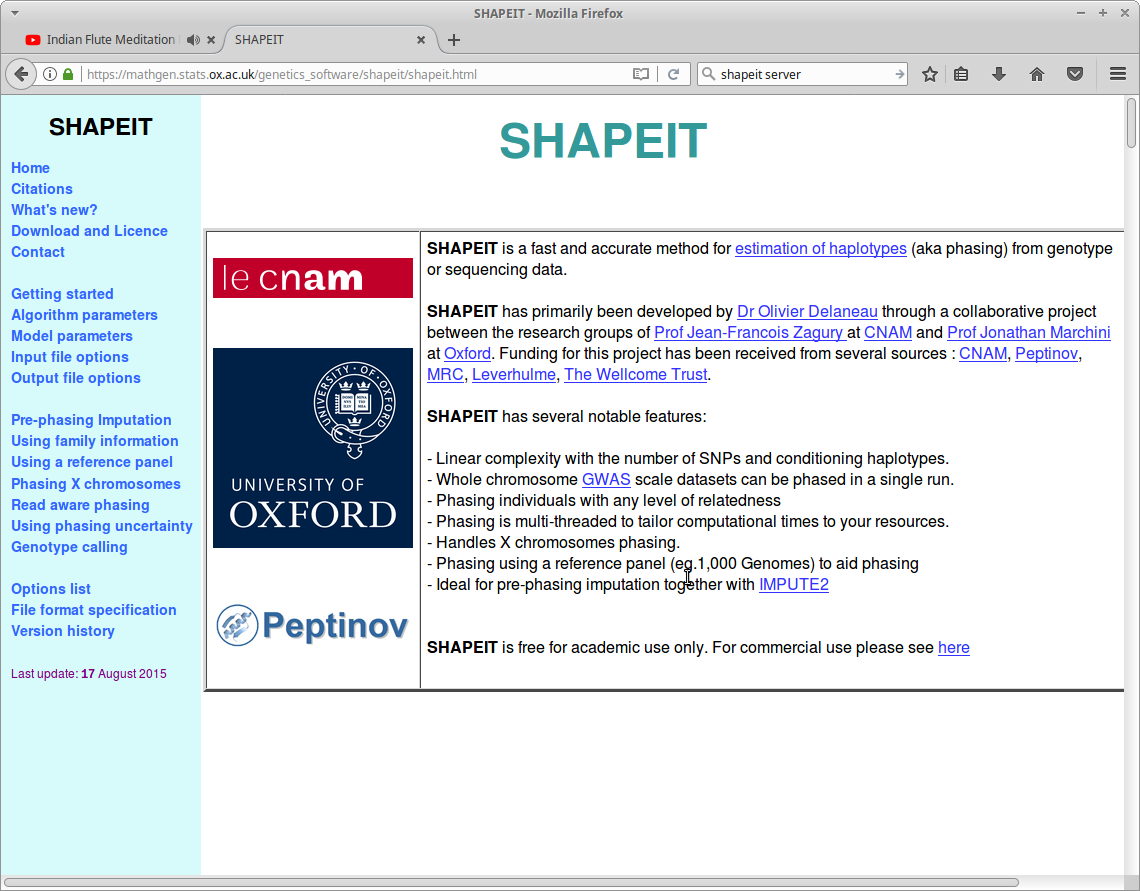
\includegraphics[width=.5\linewidth]{shapeit.png}
\end{center}
\end{figure}

\end{frame}

\begin{frame}
\frametitle{Imputaci\'on}
La imputaci\'on es un modelo probabilistico que predice cual ser\'ia los valores de un
SNP para cada sujeto de nuestra muestra, si hemos genotipado otro SNP vecino que
pretenezca al mismo bloque de LD.

\begin{figure}[htbp]
\begin{center}
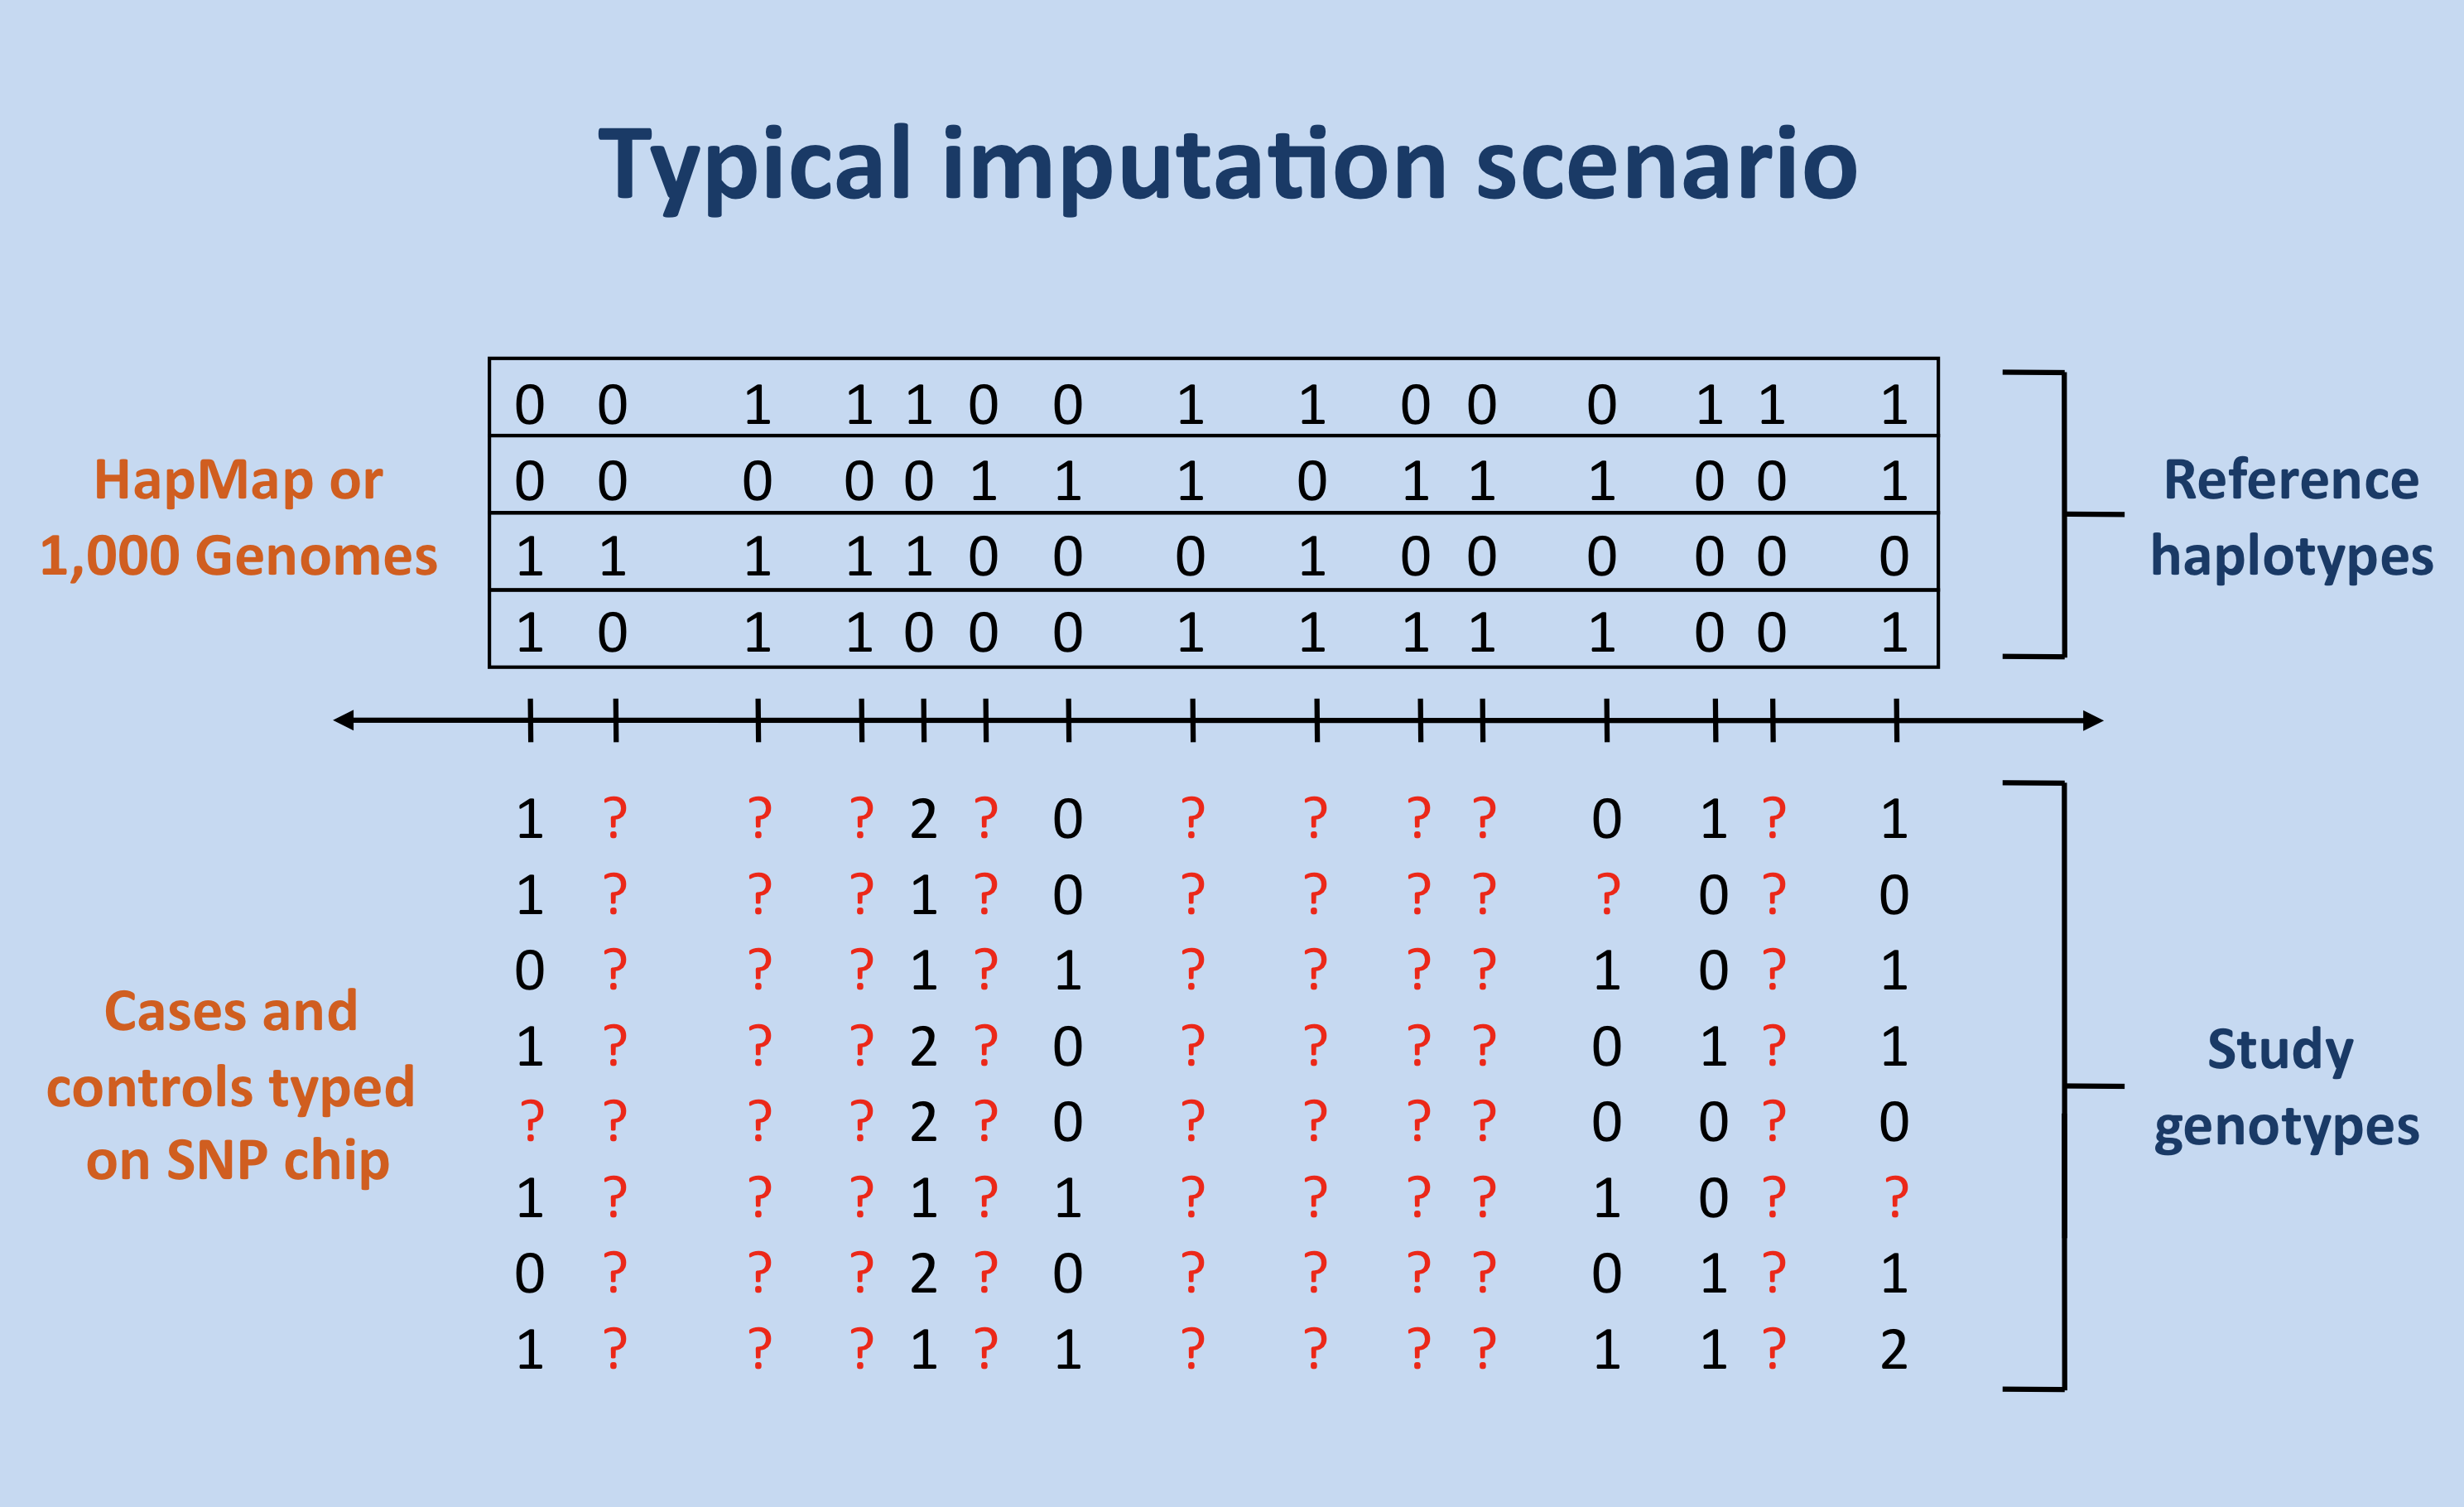
\includegraphics[width=.5\linewidth]{scenarioA.png}
\end{center}
\end{figure}

\end{frame}



\begin{frame}[fragile]
\frametitle{Imputaciones}

Hay dos softwares recomendados para hacer las imputaciones

\begin{itemize}
\item MACH: {\scriptsize {\tt http://www.sph.umich.edu/csg/abecasis/MACH/tour/imputation.html}}
de la universidad de Michigan USA
\item IMPUTE2: {\tt http://mathgen.stats.ox.ac.uk/impute/impute\_v2.html}
de la universidad de Oxford UK
\end{itemize}

Ambos corren en plataforma LINUX por linea de comandos. Por el momento no haremos practicas sobre esto, pero en la parte de Amazon computing veremos como crear un servidor LINIUX y ejecutar comandos. 

\end{frame}


\begin{frame}[fragile]
\frametitle{Imputaciones}
IMPUTE2 usa SHEPEIT para prefasear los datos

\begin{figure}[htbp]
\begin{center}
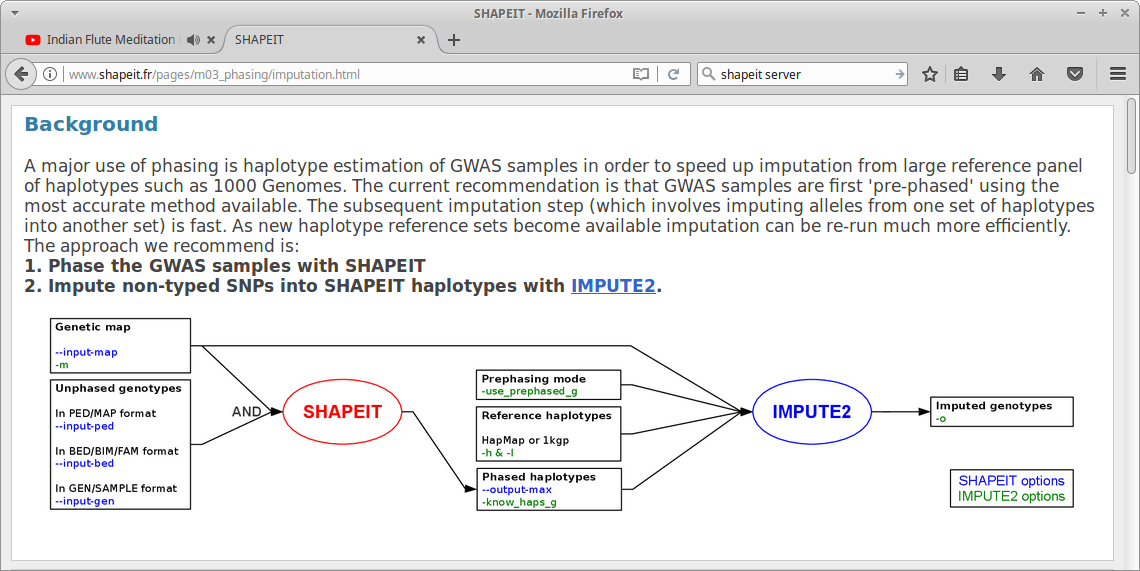
\includegraphics[width=.5\linewidth]{impute.png}
\end{center}
\end{figure}

\end{frame}

\begin{frame}[fragile]
\frametitle{Imputaciones}
La universidad de Michigan ofrece un servidor para hacer las imputaciones con diferentes paneles de referencia

\begin{figure}[htbp]
\begin{center}
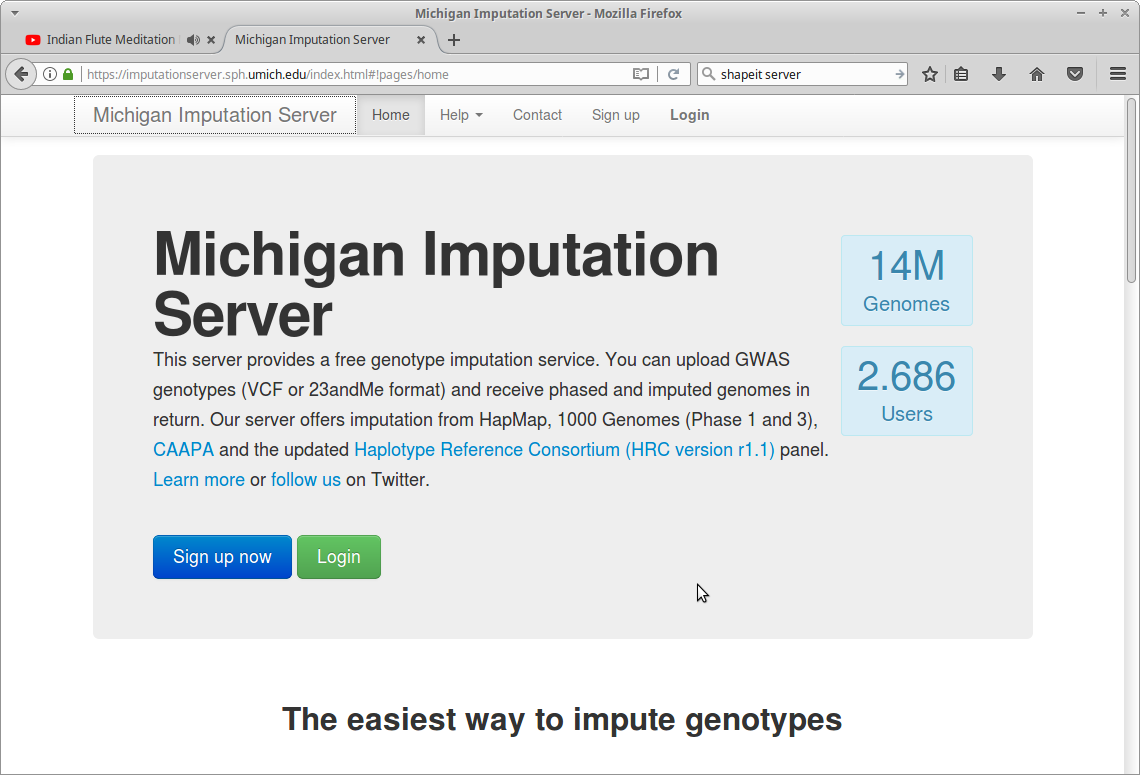
\includegraphics[width=.5\linewidth]{michigan.png}
\end{center}
\end{figure}

\begin{itemize}
\item Tienen gu\'ias detalladas para procesar los datos antes de subirlos
\item Es gratis pero va hay que ponerse en la cola 
\end{itemize}

\end{frame}


\end{document}
